\documentclass[letterpaper]{article}
%\documentclass[a4paper]{article}
\usepackage{Sweave}
\usepackage{amsmath}
\usepackage[round]{natbib}
%\usepackage{hyperref}
%\usepackage{url}
%\usepackage[left=2.5cm,right=2.5cm,top=2.5cm]{geometry}
\usepackage{geometry}

%% headings ========================================================
\pagestyle{myheadings} \markright{\hfill Bayesian Screening and Model
Discrimination \hfill}
%% headings ========================================================


\begin{document}
%\VignetteIndexEntry{Bayesian Screening and Model Discrimination}
%\VignetteDepends{BsMD}

\setkeys{Gin}{width=\textwidth}
\title{Using the \textsf{BsMD} Package for Bayesian Screening and Model Discrimination}
\author{Ernesto Barrios\\Center for Quality and Productivity Improvement\\
  University of Wisconsin-Madison}
\date{}
\maketitle
\tableofcontents

\section{Introduction}

Screening experiments are employed the at initial stages of investigation to
discriminate, among many factors, those with potential effect over the
response under study. It is common in screening studies to use most of the
observations estimating different contrasts, leaving only a few or even no
degrees of freedom at all to estimate the experiment standard error. Under
these conditions it is not possible to assess the statistical significance
of the estimated contrast effects. Some procedures, for example, the
analysis of the normal plot of the effects, have been developed to overcome
this situation.

\textsf{BsMD} package includes a set of functions useful for factor screening
in unreplicated factorial experiments. Some of the functions were written
originally for \textsf{S}, then adapted for \textsf{S-PLUS} and now for
\textsf{R}. Functions for Bayesian screening and model discrimination
follow-up designs are based on Daniel Meyer's \textsf{mdopt}
\textsc{fortran} bundle \citep{Meyer-1996}. The programs were modified and
converted to subroutines to be called from \textsf{R} functions.


This document is organized in three sections: Screening Designs, Bayesian
Screening, and Model Discrimination, with the references to the articles as
subsections to indicate the sources of the examples presented. All the
examples in \citet{Box&Meyer-1986,Box&Meyer-1993} and
\citet*{Meyer&etal-1996} are worked out and the code displayed in its
totality to show the use of the functions in the \textsf{BsMD} package. The
detailed discussion of the examples and the theory behind them is left to the
original papers. Details of the \textsf{BsMD} functions are contained to
their help pages.


\section{Screening Designs\label{sec:ScreeningDesigns}}

In screening experiments, \emph{factor sparsity} is usually assumed. That is,
from all factors considered in the experiment only a few of these will
actually affect the response. (See for example, \citet{Box&Meyer-1986}, sec.
1.) Based on this sparsity hypothesis various procedures have have been
developed to identify such active factors. Some of these procedures are
included in the \textsf{BsMD} package: \texttt{DanielPlot} (Normal Plot of
Effects), \texttt{LenthPlot} (based on a robust estimation of the standard
error of the contrasts), and \texttt{BsProb} for Bayesian screening. See the
references for details on the theory of the procedures. The data set used in
the examples of this section is from \citet{Box&Meyer-1986}. They represent
four different experiments: \emph{log drill advance}, \emph{tensile
strength}, \emph{shrinkage} and \emph{yield of isatin} with responses denoted
by \texttt{y1},\dots,\texttt{y4} and different design factors. The estimable
contrasts are denoted by \texttt{X1},\dots,\texttt{X15}. The design matrix
and responses are presented next.

\begin{Schunk}
\begin{Sinput}
> options(width = 80)
> library(BsMD)
> data(BM86.data, package = "BsMD")
> print(BM86.data)
\end{Sinput}
\begin{Soutput}
   X1 X2 X3 X4 X5 X6 X7 X8 X9 X10 X11 X12 X13 X14 X15   y1   y2   y3   y4
1  -1 -1  1 -1  1  1 -1 -1  1   1  -1   1  -1  -1   1 0.23 43.7 14.0 0.08
2   1 -1 -1 -1 -1  1  1 -1 -1   1   1   1   1  -1  -1 0.30 40.2 16.8 0.04
3  -1  1 -1 -1  1 -1  1 -1  1  -1   1   1  -1   1  -1 0.52 42.4 15.0 0.53
4   1  1  1 -1 -1 -1 -1 -1 -1  -1  -1   1   1   1   1 0.54 44.7 15.4 0.43
5  -1 -1  1  1 -1 -1  1 -1  1   1  -1  -1   1   1  -1 0.70 42.4 27.6 0.31
6   1 -1 -1  1  1 -1 -1 -1 -1   1   1  -1  -1   1   1 0.76 45.9 24.0 0.09
7  -1  1 -1  1 -1  1 -1 -1  1  -1   1  -1   1  -1   1 1.00 42.2 27.4 0.12
8   1  1  1  1  1  1  1 -1 -1  -1  -1  -1  -1  -1  -1 0.96 40.6 22.6 0.36
9  -1 -1  1 -1  1  1 -1  1 -1  -1   1  -1   1   1  -1 0.32 42.4 22.3 0.79
10  1 -1 -1 -1 -1  1  1  1  1  -1  -1  -1  -1   1   1 0.39 45.5 17.1 0.68
11 -1  1 -1 -1  1 -1  1  1 -1   1  -1  -1   1  -1   1 0.61 43.6 21.5 0.73
12  1  1  1 -1 -1 -1 -1  1  1   1   1  -1  -1  -1  -1 0.66 40.6 17.5 0.08
13 -1 -1  1  1 -1 -1  1  1 -1  -1   1   1  -1  -1   1 0.89 44.0 15.9 0.77
14  1 -1 -1  1  1 -1 -1  1  1  -1  -1   1   1  -1  -1 0.97 40.2 21.9 0.38
15 -1  1 -1  1 -1  1 -1  1 -1   1  -1   1  -1   1  -1 1.07 42.5 16.7 0.49
16  1  1  1  1  1  1  1  1  1   1   1   1   1   1   1 1.21 46.5 20.3 0.23
\end{Soutput}
\end{Schunk}

Saturated linear models for each of the responses are fitted and the
estimated coefficients are presented in the table below. The \texttt{lm}
calls, not displayed here, produce the \texttt{advance.lm}, \dots,
\texttt{yield.lm} objects used in the next subsections.

\begin{Schunk}
\begin{Soutput}
            advance shrinkage strength yield
(Intercept)    0.70     42.96    19.75  0.38
X1             0.03      0.06    -0.30 -0.10
X2             0.13     -0.07    -0.20 -0.01
X3            -0.01      0.15    -0.30  0.00
X4             0.25      0.08     2.30 -0.04
X5             0.00      0.20     0.45  0.02
X6            -0.01     -0.01    -0.10 -0.03
X7             0.00      0.19    -0.15  0.07
X8             0.07      0.20    -0.60  0.14
X9             0.01     -0.03     0.35 -0.08
X10            0.00      0.21     0.05 -0.13
X11            0.01      0.06     0.15 -0.05
X12            0.02      0.06    -2.75 -0.01
X13            0.01     -0.19     1.90  0.00
X14           -0.01      1.07     0.05  0.06
X15            0.01      1.55    -0.30  0.01
\end{Soutput}
\end{Schunk}

For each of the experiments the 16 runs are used on the estimation of the 15
contrasts and the constant term. Thus the need of graphical aims to determine
which are likely active contrasts.

\subsection{Daniel Plots}
Daniel plots, known as normal plot of effects, arrange the estimated factor
effects in a normal probability plot; those factors ``out of the straight
line'' are identified as potentially active factors. See for example,
\cite{Daniel-1976} for different applications and interpretations.

\texttt{DanielPlot} produces normal plot of effects. The main argument of the
function is an \texttt{lm} object, say, \texttt{lm.obj}. The function removes
the constant term \texttt{(Intercept)} if it is in the model. Factor effects,
assumed as \texttt{2*coef(lm.obj)} are displayed using the \texttt{qqnorm}
function. See the help pages for details.

\subsubsection{Box et al. 1986: Example 1}
By default \texttt{DanielPlot} labels all the effects, as show in figure a).
This example shows how to label only some particular factors for clarity, as
exhibited in figure b). The corresponding linear model \texttt{advance.lm}
was already fitted at the beginning of the section.

\begin{center}
\begin{Schunk}
\begin{Sinput}
> par(mfrow = c(1, 2), mar = c(3, 3, 1, 1), mgp = c(1.5, 0.5, 0), 
+     oma = c(0, 0, 0, 0), xpd = TRUE, pty = "s", cex.axis = 0.7, 
+     cex.lab = 0.8, cex.main = 0.9)
> DanielPlot(advance.lm, cex.pch = 0.8, main = "a) Default Daniel Plot")
> DanielPlot(advance.lm, cex.pch = 0.8, main = "b) Labelled Plot", 
+     pch = 20, faclab = list(idx = c(2, 4, 8), lab = c(" 2", " 4", 
+         " 8")))
\end{Sinput}
\end{Schunk}
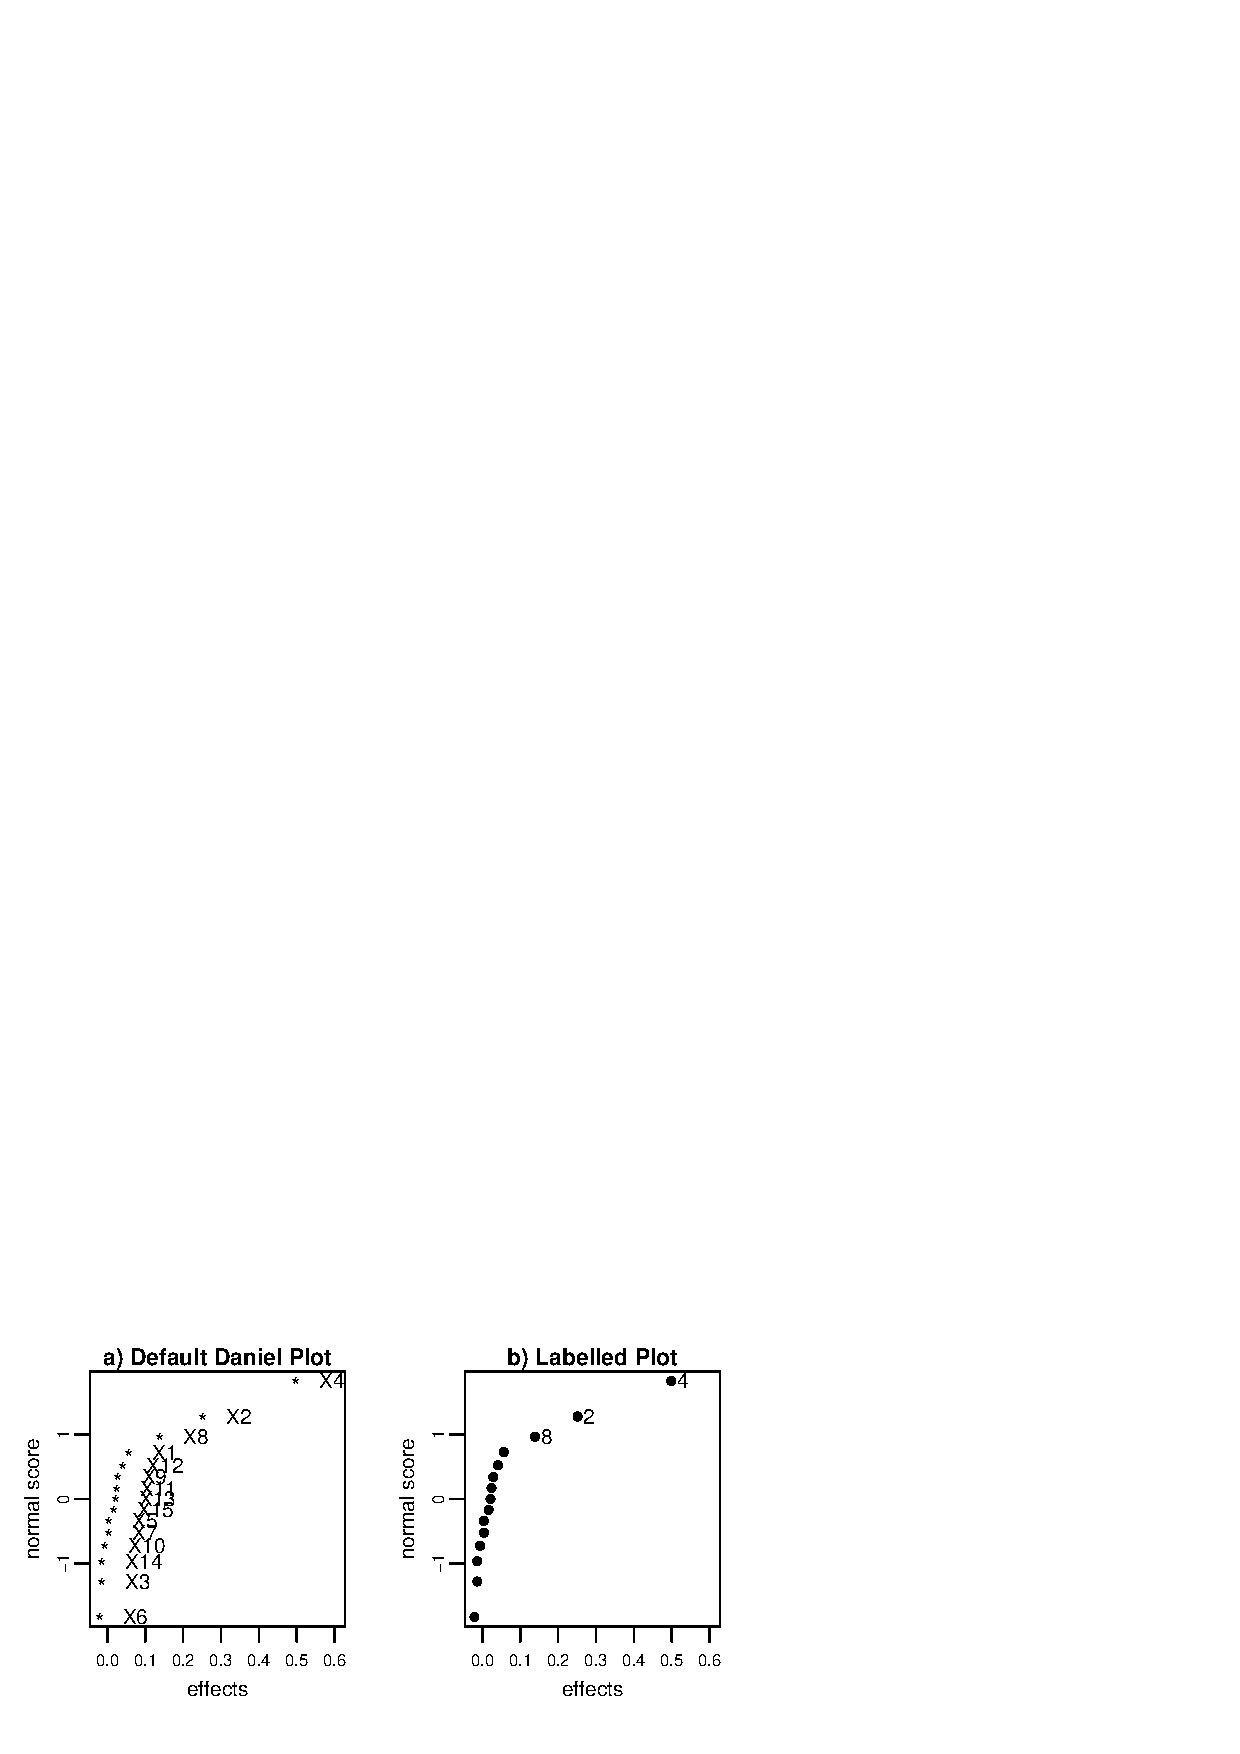
\includegraphics{BsMD-DanielPlots}
\end{center}

\subsubsection{Box et al. 1986: Example 3}

Some people prefer the use of half-normal plots. These plots are similar to
the normal plots but instead of the signed effects absolute values of the
effects are displayed. There are some advantages and disadvantages using one
or the other. See for example, \citet[chap.~7.6]{Daniel-1976}.

Figure a) depicts the half-normal plot of the effects for the strength
response (\texttt{y3}). \texttt{DanielPlot} has the option to generate
half-normal plots (\texttt{half=TRUE}). The corresponding normal plot of
signed effects is presented in figure b) below.

\begin{center}
\begin{Schunk}
\begin{Sinput}
> par(mfrow = c(1, 2), mar = c(3, 3, 1, 1), mgp = c(1.5, 0.5, 0), 
+     oma = c(0, 0, 0, 0), xpd = TRUE, pty = "s", cex.axis = 0.7, 
+     cex.lab = 0.8, cex.main = 0.9)
> DanielPlot(strength.lm, half = TRUE, cex.pch = 0.8, main = "a) Half-Normal Plot", 
+     faclab = list(idx = c(4, 12, 13), lab = c(" x4", " x12", 
+         " x13")))
> DanielPlot(strength.lm, main = "b) Normal Plot", faclab = list(idx = c(4, 
+     12, 13), lab = c(" 4", " 12", " 13")))
\end{Sinput}
\end{Schunk}
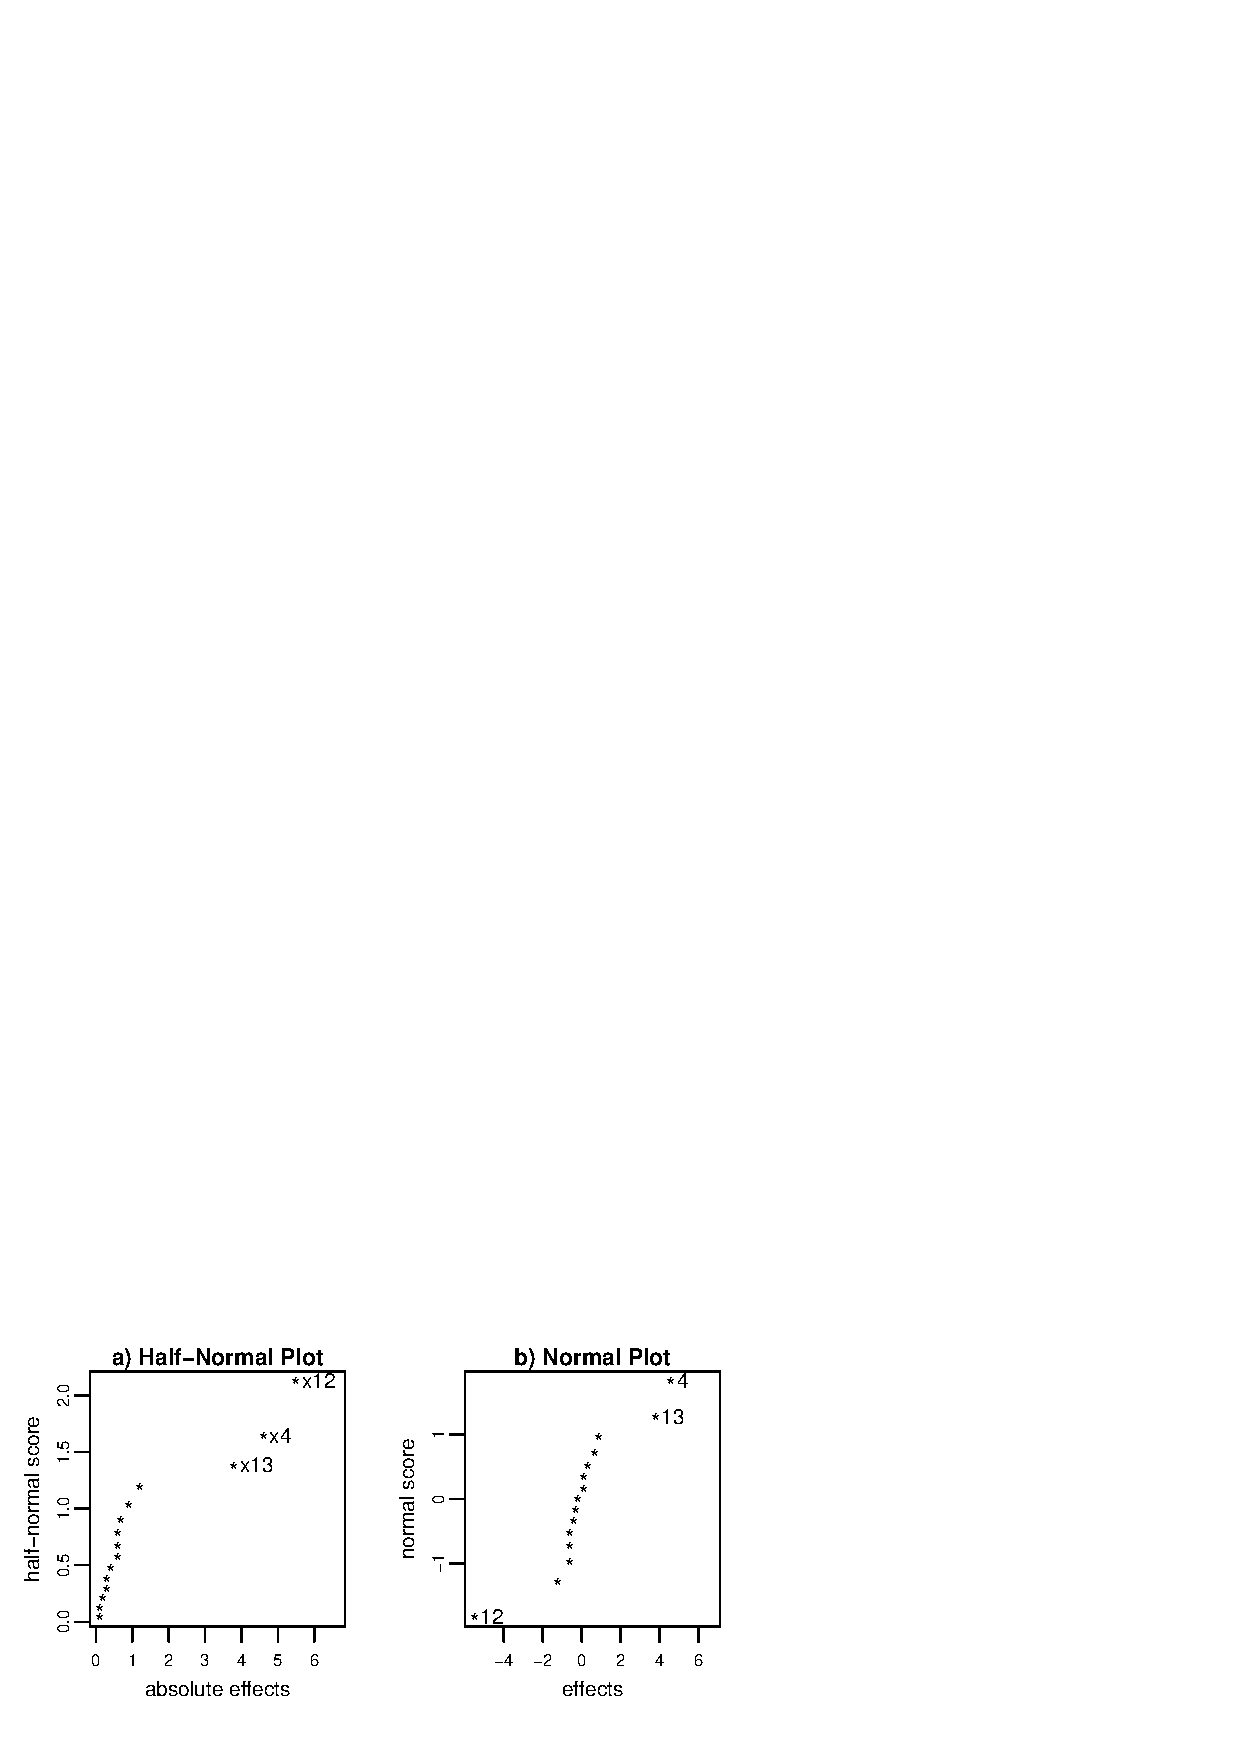
\includegraphics{BsMD-004}
\end{center}

\subsection{Lenth Plots}

Lenth's method for factor effects assessment is based on factor sparsity too.
For and unreplicated factorial design Let $c_1,\dots,c_m$ the estimated
contrasts and approximate the standard error by \( s_0 = 1.5 \times
\mathop{\text{median}} |c_i| \). Then the author defines the \emph{pseudo
standard error} by
\[ \text{PSE}=1.5 \times \mathop{\text{median}}_{|c_j|<2.5s_0} |c_j| \]
and the 95\% \emph{margin of error} by
\[ \text{ME}=t_{0.975,d} \times \text{PSE} \]
where $t_{0.975,d}$ is the .975th quantile of the $t$ distribution with
$d=m/3$ degrees of freedom. The 95\% \emph{simultaneous margin of error}
(SME) is defined for simultaneous inference on all the contrast and is given
by
\[\text{SME} = t_{\gamma,d} \times \text{PSE} \]
where $\gamma=(1+0.95^{1/m})/2$.  See \citet{Lenth-1989}, for details.

The \texttt{LenthPlot} function displays the factor effects and the SE and
SME limits. Spikes instead of the barplot used originally by Lenth are
employed to represent the factor effects. As in \texttt{DanielPlot}, the main
argument for the function is a \texttt{lm} object, and
\texttt{2*coef(lm.obj)} is displayed.

\subsubsection{Box et al. 1986: Example 2}

Figure a) below shows the default plot produced by \texttt{LenthPlot}. The SE
and MSE limits at a 95\% confidence level ($\alpha=0.05$) are displayed by
default. Figure b) shows Lenth's plot for the same experiment using
$\alpha=0.01$, locating the labels of SME and ME close to the vertical axis
and labelling the contrast effects $X_{14}$ and $X_{15}$ as $P$ and $-M$, for
period and material respectively and accordingly to Lenth's paper. Note that
the effects are considered as 2 times the coefficients $\texttt{b}$.

\begin{center}
\begin{Schunk}
\begin{Sinput}
> par(mfrow = c(1, 2), mar = c(4, 4, 1, 1), mgp = c(1.5, 0.5, 0), 
+     oma = c(0, 0, 0, 0), xpd = TRUE, pty = "s", cex.axis = 0.7, 
+     cex.lab = 0.8, cex.main = 0.9)
> LenthPlot(shrinkage.lm)
\end{Sinput}
\begin{Soutput}
    alpha       PSE        ME       SME 
0.0500000 0.2250000 0.5783809 1.1741965 
\end{Soutput}
\begin{Sinput}
> title("a) Default Lenth Plot")
> b <- coef(shrinkage.lm)[-1]
> LenthPlot(shrinkage.lm, alpha = 0.01, adj = 0.2)
\end{Sinput}
\begin{Soutput}
    alpha       PSE        ME       SME 
0.0100000 0.2250000 0.9072322 1.6855749 
\end{Soutput}
\begin{Sinput}
> title(substitute("b) Lenth Plot (" * a * ")", list(a = quote(alpha == 
+     0.01))))
> text(14, 2 * b[14], "P ", adj = 1, cex = 0.7)
> text(15, 2 * b[15], " -M", adj = 0, cex = 0.7)
\end{Sinput}
\end{Schunk}
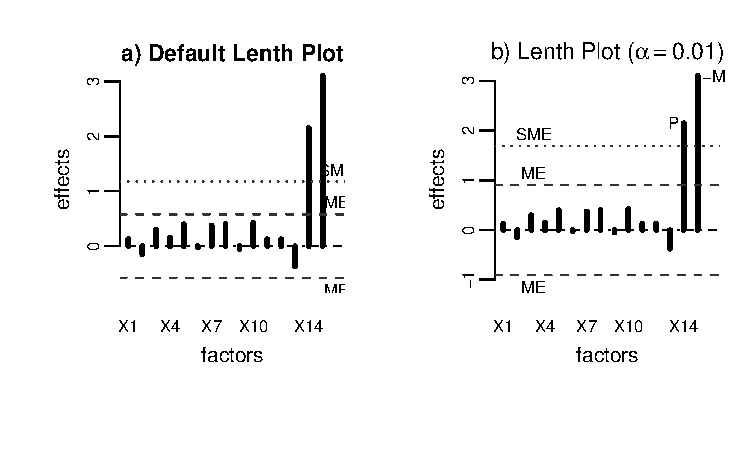
\includegraphics{BsMD-005}
\end{center}

\subsubsection{Box et al. 1986: Example 4\label{sec:isatin}}
This example exhibits the Daniel and Lenth plots for the isatin data,
originally presented by Davis and co-authors in 1954 and discussed in the Box
and Meyer paper (p. 16--17). As can be seen in the figures below, it is not
clear which contrasts may be active. For example, in Lenth's plot none of the
effects goes beyond the margin of error ME, thus the SME limits are not
displayed. The corresponding Bayes plot is presented in the next section.

\begin{center}
\begin{Schunk}
\begin{Sinput}
> par(mfrow = c(1, 2), mar = c(3, 3, 1, 1), mgp = c(1.5, 0.5, 0), 
+     oma = c(0, 0, 0, 0), pty = "s", cex.axis = 0.7, cex.lab = 0.8, 
+     cex.main = 0.9)
> DanielPlot(yield.lm, cex.pch = 0.6, main = "a) Daniel Plot")
> LenthPlot(yield.lm, alpha = 0.05, xlab = "factors", adj = 0.9, 
+     main = "b) Lenth Plot")
\end{Sinput}
\begin{Soutput}
    alpha       PSE        ME       SME 
0.0500000 0.1143750 0.2940103 0.5968832 
\end{Soutput}
\end{Schunk}
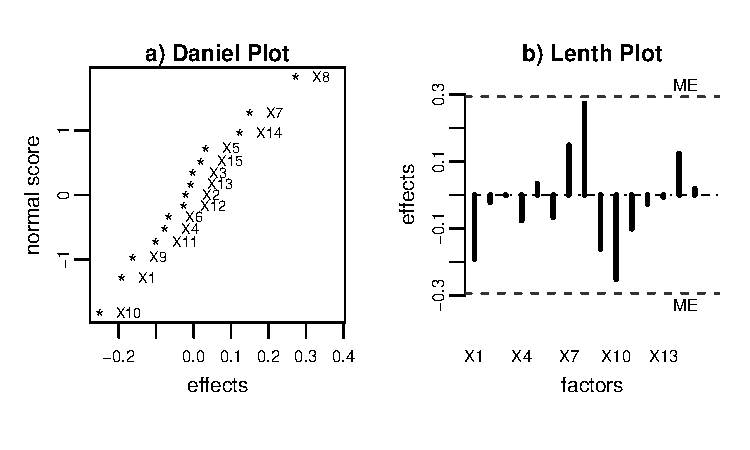
\includegraphics{BsMD-006}
\end{center}

\section{Bayesian Screening}

Box and Meyer Bayesian screening is also based on the factor sparsity
hypothesis. For the linear model $y=X\beta+\epsilon$, the procedure assigns
to each of the $\beta_i$ independent prior normal distributions
$N(0,\gamma^2\sigma^2)$, where $\sigma^2$ is the variance of the error and
$\gamma^2$ is the magnitude of the effect relative to the experimental noise.
The factor sparsity assumption is brought into the procedure assigning a
prior probability $\pi$ to any factor of being active, and $1-\pi$ to the
factor of being inert. Models $M_l$ for all-subsets of factors (main effects
and interactions) are constructed and their posterior probabilities
calculated. Marginal factor posterior probabilities $p_i$ are computed and
displayed. Those contrasts or factor effects with higher probabilities are
identified as potentially active. See \citet{Box&Meyer-1986,Box&Meyer-1993}
for explanation and details of the procedure.

The \texttt{BsProb} function computes the posterior probabilities for
Bayesian screening. The function calls the \texttt{bs} \textsc{fortran}
subroutine, a modification of the \texttt{mbcqpi5.f} program included in the
\textsf{mdopt} bundle. The complete output of the program is saved in the
working directory as \texttt{BsPrint.out}. The file is overwritten if it
already exists. Thus, rename the \texttt{BsPrint.out} file after each call to
\texttt{BsProb} if you want to keep the complete output. Note however, that
most of the output is included in the \texttt{BsProb}'s output list. This is
a list of class \texttt{BsProb} with methods functions for \texttt{print},
\texttt{plot} and \texttt{summary}.

\subsection{Fractional Factorial Designs}

Bayesian screening was presented by Box and Meyer in their 1986 and 1993
papers. The former refers to 2-level orthogonal designs while the latter
refer to general designs. The distinction is important since in the case of
2-level orthogonal designs some factorization is possible that allows the
calculation of the marginal probabilities without summing over all-subsets
models' probabilities. This situation is explained in the 1986 paper, where
$\alpha$ and $k$ are used instead of the $\pi$ and $\gamma$ described at the
beginning of the section. Their correspondence is $\alpha=\pi$, and
$k^2=n\gamma^2+1$, where $n$ is the number of runs in the design. The
function is written for the general case and arguments \texttt{p} and
\texttt{g} (for $\pi$ and $\gamma$) should be provided. In the mentioned
paper the authors estimated $\alpha$ and $k$ for a number of published
examples. They found $.13\leq \hat{\alpha} \leq .27$, and $2.7\leq
\hat{k}\leq 27$. Average values of $\alpha=0.20\ (=\pi)$ and $k=10\
(\gamma=2.49)$ are used in the examples.

\subsubsection{Box et al. 1986: Example 1}

This example exhibits most of the output of the \texttt{BsProb} function. The
design matrix and response vector, the 15 contrasts and 5 models posterior
probabilities are printed. As mentioned before, \texttt{g=2.49} corresponds
to $k=10$ used in the paper. Note that all possible $2^{15}$ factor
combinations were used to construct the \texttt{totMod=32768} estimated
models. Only the top \texttt{nMod=5} are displayed. See the \texttt{BsProb}
help pages for details. Figures below show the Bayes plot (a) and Daniel plot
(b) for the estimated effects. In this case both procedures clearly identify
$x_2$, $x_4$, and $x_8$ as active contrasts.

\begin{center}
\begin{Schunk}
\begin{Sinput}
> par(mfrow = c(1, 2), mar = c(3, 3, 1, 1), mgp = c(1.5, 0.5, 0), 
+     oma = c(0, 0, 0, 0), pty = "s", cex.axis = 0.7, cex.lab = 0.8, 
+     cex.main = 0.9)
> X <- as.matrix(BM86.data[, 1:15])
> y <- BM86.data[, 16]
> advance.BsProb <- BsProb(X = X, y = y, blk = 0, mFac = 15, mInt = 1, 
+     p = 0.2, g = 2.49, ng = 1, nMod = 10)
> print(advance.BsProb, X = FALSE, resp = FALSE, nMod = 5)
\end{Sinput}
\begin{Soutput}
 Calculations:
    nRun     nFac     nBlk     mFac     mInt        p        g   totMod 
   16.00    15.00     0.00    15.00     1.00     0.20     2.49 32768.00 

 Output file: BsPrint.out

 Factor probabilities:
   Factor Code  Prob
1    none none 0.000
2      X1   x1 0.240
3      X2   x2 1.000
4      X3   x3 0.028
5      X4   x4 1.000
6      X5   x5 0.025
7      X6   x6 0.034
8      X7   x7 0.025
9      X8   x8 0.983
10     X9   x9 0.046
11    X10  x10 0.025
12    X11  x11 0.037
13    X12  x12 0.091
14    X13  x13 0.034
15    X14  x14 0.028
16    X15  x15 0.030

 Model probabilities:
   Prob  Sigma2 NumFac Factors   
M1 0.504 0.003  3      2,4,8     
M2 0.148 0.002  4      1,2,4,8   
M3 0.043 0.003  4      2,4,8,12  
M4 0.022 0.003  4      2,4,8,9   
M5 0.022 0.002  5      1,2,4,8,12
\end{Soutput}
\begin{Sinput}
> plot(advance.BsProb, main = "a) Bayes Plot")
> DanielPlot(advance.lm, cex.pch = 0.6, main = "b) Daniel Plot", 
+     faclab = list(idx = c(2, 4, 8), lab = c(" x2", " x4", " x8")))
\end{Sinput}
\end{Schunk}
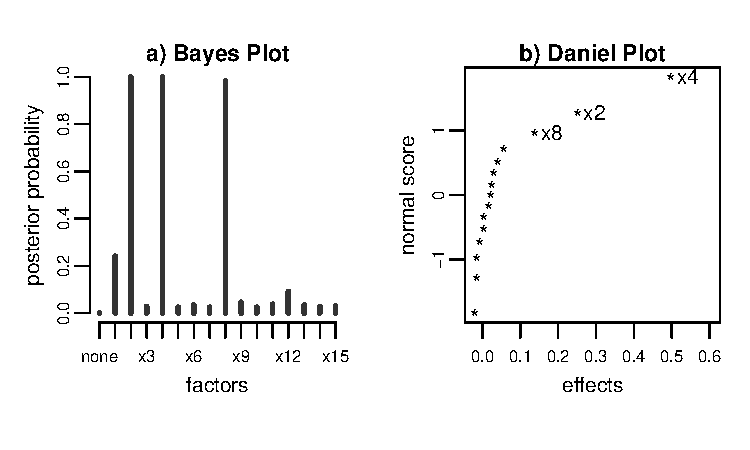
\includegraphics{BsMD-007}
\end{center}

\subsubsection{Box et al. 1986: Example 4}

As mentioned in section~\ref{sec:isatin}, in the isatin data example active
contrasts, if present, are not easily identified by Daniel or Lenth's plot.
This situation is reflected in the sensitivity of the Bayes procedure to the
value of $\gamma$. Different values for $k$ ($\gamma$) can be provided to the
\texttt{BsProb} function and the respective factor posterior probabilities
computed. The range of such probabilities is plotted as stacked spikes. This
feature is useful in data analysis. See next subsection for further
explanation. In the call of the function \textsf{BsProb},
\texttt{g=c(1.22,3.74)} and \texttt{ng=10} indicate that the calculation of
the marginal posterior probabilities is done for 10 equally spaced values of
$\gamma$ in the range $(1.22, 3.74)$ corresponding to the range of $k$
between 5 and 15 used in the paper. The sensitivity of the posterior
probabilities to various values of $\gamma$ is exhibited in figure a) below.
The large ranges displayed by some of the contrasts is an indication that no
reliable inference is possible to draw from the data.

\begin{center}
\begin{Schunk}
\begin{Sinput}
> par(mfrow = c(1, 2), mar = c(3, 3, 1, 1), mgp = c(1.5, 0.5, 0), 
+     oma = c(0, 0, 0, 0), pty = "s", cex.axis = 0.7, cex.lab = 0.8, 
+     cex.main = 0.9)
> X <- as.matrix(BM86.data[, 1:15])
> y <- BM86.data[, 19]
> yield.BsProb <- BsProb(X = X, y = y, blk = 0, mFac = 15, mInt = 1, 
+     p = 0.2, g = c(1.22, 3.74), ng = 10, nMod = 10)
> summary(yield.BsProb)
\end{Sinput}
\begin{Soutput}
 Calculations:
    nRun     nFac     nBlk     mFac     mInt        p     g[1]    g[10] 
   16.00    15.00     0.00    15.00     1.00     0.20     1.22     3.74 
  totMod 
32768.00 

 Posterior probabilities for each gamma value:
          1     2     3     4     5     6     7     8     9    10
gamma 1.220 1.500 1.780 2.060 2.340 2.620 2.900 3.180 3.460 3.740
none  0.120 0.167 0.218 0.268 0.316 0.360 0.400 0.436 0.469 0.498
x1    0.314 0.271 0.228 0.190 0.159 0.134 0.115 0.099 0.086 0.076
x2    0.049 0.041 0.035 0.030 0.027 0.024 0.022 0.020 0.018 0.017
x3    0.048 0.039 0.034 0.029 0.026 0.023 0.021 0.019 0.018 0.016
x4    0.074 0.066 0.059 0.053 0.048 0.042 0.037 0.032 0.028 0.025
x5    0.051 0.043 0.037 0.032 0.028 0.026 0.023 0.021 0.019 0.018
x6    0.066 0.057 0.051 0.047 0.042 0.038 0.034 0.030 0.027 0.024
x7    0.196 0.170 0.143 0.119 0.099 0.083 0.070 0.060 0.052 0.045
x8    0.588 0.531 0.473 0.420 0.374 0.335 0.302 0.274 0.250 0.230
x9    0.228 0.197 0.164 0.136 0.113 0.095 0.080 0.069 0.060 0.052
x10   0.513 0.456 0.399 0.348 0.304 0.267 0.237 0.212 0.191 0.173
x11   0.104 0.093 0.082 0.071 0.061 0.052 0.045 0.039 0.034 0.030
x12   0.050 0.041 0.035 0.031 0.027 0.024 0.022 0.020 0.019 0.017
x13   0.048 0.040 0.034 0.029 0.026 0.023 0.021 0.019 0.018 0.016
x14   0.142 0.125 0.107 0.091 0.076 0.064 0.055 0.047 0.041 0.035
x15   0.049 0.040 0.034 0.030 0.026 0.024 0.021 0.020 0.018 0.017
\end{Soutput}
\begin{Sinput}
> plot(yield.BsProb, main = "a) Bayes Plot")
> title(substitute("( " * g1 * "" * g2 * " )", list(g1 = quote(1.2 <= 
+     gamma), g2 = quote("" <= 3.7))), line = -1)
> DanielPlot(yield.lm, cex.pch = 0.6, main = "b) Daniel Plot", 
+     faclab = list(idx = c(1, 7, 8, 9, 10, 14), lab = paste(" ", 
+         c(1, 7, 8, 9, 10, 14), sep = "")))
\end{Sinput}
\end{Schunk}
